\documentclass[12pt]{article}
\usepackage[utf8]{inputenc}

\usepackage{lmodern}

\usepackage{enumitem}
\usepackage[margin=2cm]{geometry}

\usepackage{amsmath, amsfonts, amssymb}
\usepackage{graphicx}
%\usepackage{subfigure}
\usepackage{tikz}
\usepackage{pgfplots}
\usepackage{multicol}

\usepackage{comment}
\usepackage{url}
\usepackage{calc}
\usepackage{subcaption}
\usepackage[indent=0pt]{parskip}
\usepackage{animate}

\usepackage{array}
\usepackage{blkarray,booktabs, bigstrut}
\usepackage{bigints}

\pgfplotsset{compat=1.16}

% MATH commands
\newcommand{\ga}{\left\langle}
\newcommand{\da}{\right\rangle}
\newcommand{\oa}{\left\lbrace}
\newcommand{\fa}{\right\rbrace}
\newcommand{\oc}{\left[}
\newcommand{\fc}{\right]}
\newcommand{\op}{\left(}
\newcommand{\fp}{\right)}

\newcommand{\bi}{\mathbf{i}}
\newcommand{\bj}{\mathbf{j}}
\newcommand{\bk}{\mathbf{k}}
\newcommand{\bF}{\mathbf{F}}

\newcommand{\mR}{\mathbb{R}}

\newcommand{\ra}{\rightarrow}
\newcommand{\Ra}{\Rightarrow}

\newcommand{\sech}{\mathrm{sech}\,}
\newcommand{\csch}{\mathrm{csch}\,}
\newcommand{\curl}{\mathrm{curl}\,}
\newcommand{\dive}{\mathrm{div}\,}

\newcommand{\ve}{\varepsilon}
\newcommand{\spc}{\vspace*{0.5cm}}

\DeclareMathOperator{\Ran}{Ran}
\DeclareMathOperator{\Dom}{Dom}

\newcommand{\exo}[1]{\noindent\textcolor{red}{\fbox{\textbf{Problem {#1}}}\hrulefill}\\\\ }
\newcommand{\qu}[4]{\noindent\textcolor{#4}{\fbox{\textbf{Section {#1} | Problem {#2}}} \hrulefill{{\fbox{\textbf{{#3} Points}}}}\\}}

\newcommand{\semester}{Fall 2023}

\newcommand{\CVup}{%
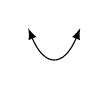
\begin{tikzpicture}
\draw[black, <->, >=latex] (-0.33, 0.5) .. controls (-0.125, 0) and (0.125, 0) .. (0.33, 0.5);
\end{tikzpicture}}

\newcommand{\CVupInc}{%
\begin{tikzpicture}
\draw[black, ->, >=latex] (0,0) .. controls (0.2, 0) and (0.4, 0.2) .. (0.5, 0.5);
\end{tikzpicture}}

\newcommand{\CVupDec}{%
\begin{tikzpicture}[rotate=270]
\draw[black, ->, >=latex] (0,0) .. controls (0.2, 0) and (0.4, 0.2) .. (0.5, 0.5);
\end{tikzpicture}}

\newcommand{\CVdown}{%
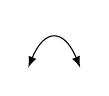
\begin{tikzpicture}
\draw[black, <->, >=latex] (-0.33, -0.5) .. controls (-0.125, 0) and (0.125, 0) .. (0.33, -0.5);
\end{tikzpicture}}

\newcommand{\CVdownInc}{%
\begin{tikzpicture}
\draw[black, ->, >=latex] (-0.5, -0.5) .. controls (-0.5, -0.3) and (-0.5, -0.1) .. (0,0);
\end{tikzpicture}}

\newcommand{\CVdownDec}{%
\begin{tikzpicture}[rotate=-90]
\draw[black, ->, >=latex] (-0.5, -0.5) .. controls (-0.5, -0.3) and (-0.5, -0.1) .. (0,0);
\end{tikzpicture}}

\begin{document}
	\noindent \hrulefill \\
	MATH-244 \semester \hfill Practice Problems Solutions\\
	Section 16.7 \hfill Pierre-Olivier Paris{\'e} \\\vspace*{-1cm}
	
	\noindent\hrulefill
	
	\spc	

	\exo{40}
	\underline{\textbf{(From Section 16.6)}}
	We have
		\begin{align*}
		\vec{r}_u &= \left\langle 1 , -3, 1 \right\rangle \\
		\vec{r}_v &= \left\langle 1, 0, -1 \right\rangle .
		\end{align*}
	So, $\vec{r}_u \times \vec{r}_v = \left\langle 3, 2, -3 \right\rangle$. Thus,
		\begin{align*}
		\iint_S \, dS = \iint_D |\vec{r}_u \times \vec{r}_v | \, dA = \int_{-1}^1 \int_0^2 \sqrt{22} \, du dv = 4 \sqrt{22} .
		\end{align*}
	Notice here that $\vec{r}_u$ and $\vec{r}_v$ are perpendicular and so the angle form between them is $\pi/2$. Hence,
		\[
			|\vec{r}_u \times \vec{r}_v| = |\vec{r}_u | |\vec{r}_v| \sin (\pi /2 ) = |\vec{r}_u| |\vec{r}_v | .
		\]
	Beware, this is not true all the time! We need the vectors $\vec{r}_u$ and $\vec{r}_v$ to be orthogonal, which is not always the case. 
	
	\exo{44}
	\underline{\textbf{(From Section 16.6)}}
	The domain $D$ of the parameters $x$, $y$ are inside the triangle. More precisely, we have
		\begin{align*}
		D = \{ (x, y) \, : \, 0 \leq x \leq 1 \text{ and } 0 \leq y \leq 1 - x \} .
		\end{align*}
	By the formula for surfaces obtained from an equation $z = f(x, y)$, we can use te following formula
		\begin{align*}
		A (S) = \iint_D \sqrt{1 + z_x^2 + z_y^2} \, dA .
		\end{align*}
	We have $z_x = -4x$ and $z_y = 1$. Thus, we obtain
		\begin{align*}
		A (S) = \int_0^1 \int_0^{1 - x} \sqrt{2 + 16x^2} \, dy dx = \sqrt{2} \int_0^1 (1 - x) \sqrt{1 + 8x^2} \, dx \approx 0.72828
		\end{align*}
		
	\spc
	
	\exo{10}
	Intersection the plane with the $xy$-plane, we get our domain:
		\begin{align*}
		D = \{ (x, y) \, : \, 0 \leq x \leq 1 \text{ and } 0 \leq y \leq 1 - x \} .
		\end{align*}
	Now, we have $z = 4 - 2x - 2y$, so that
		\begin{align*}
		dS = \sqrt{1 + z_x^2 + z_y^2} \, dA = \sqrt{1 + 4 + 4} \, dA = 3 \, dA .
		\end{align*}
	Thus we get
		\begin{align*}
		\iint_S xz \, dS = \int_0^1 \int_0^{1 - x} 3x (4 - 2x - 2y) \, dy dx = 3 \int_0^1 x (1 - x) - 2x^2 (1 - x) - x (1 - x)^2 \, dx = -1/12 .
		\end{align*}
		
	\spc
	
	\exo{16}
	In spherical coordinates, a cone is $\phi = \pi/4$. Thus, we have
		\begin{align*}
		S = \{ (\cos \theta \sin \phi , \sin \theta \sin \phi , \cos \phi ) \, : \, 0 \leq \theta \leq 2\pi \text{, } 0 \leq \phi \leq \pi/4 \} .
		\end{align*}
	We have $dS = |\vec{r}_\theta \times \vec{r}_\phi | \, dA$. So
		\begin{align*}
		\vec{r}_\theta &= \left\langle -\sin \theta \sin \phi , \cos \theta \sin \phi , 0 \right\rangle  \\
		\vec{r}_\phi &= \left\langle \cos \theta \cos \phi , \sin \theta \cos \phi , -\sin \phi \right\rangle .
		\end{align*}
	So, we these tangent vectors, we see that
		\begin{align*}
		|\vec{r}_\theta \times \vec{r}_\phi | = \sin \phi .
		\end{align*}
	Thus, $dS = \sin \phi \, dA$ and
		\begin{align*}
		\iint_S y^2 \, dS &= \int_0^{\pi/4} \int_0^{2\pi} \sin^2 \theta \sin^2 \phi \sin \phi \, d\phi d\theta \\
		&= \int_0^{\pi/4} \sin^2 \theta \, d\theta (4/3) \\
		&= (1/8)(\pi - 2) (4/3) \\
		&= \frac{\pi - 2}{6} .
		\end{align*}
		
	\spc
	
	\exo{44}
	A parametrization of the hemisphere is
		\begin{align*}
		\vec{r} (\phi , \theta ) = \left\langle 3 \cos \theta \sin \phi , 3 \sin \theta \sin \phi , 3 \cos \phi \right\rangle 
		\end{align*}
	where $0 \leq \theta \leq 2\pi$ and $0\leq \phi \leq \pi/2$. The cross product of the tangent vectors is
		\begin{align*}
		\vec{r}_\phi \times \vec{r}_\theta = \left\langle 9 \sin^2 \phi \cos \theta , 9 \sin^2 \phi \sin \theta , 9 \sin \phi \cos \phi \right\rangle = 9 \sin \phi \left\langle \cos \theta \sin \phi , \sin \theta \sin \phi , \cos \phi \right\rangle .
		\end{align*}
	 The vector $\vec{r}_\phi \times \vec{r}_\theta$ is pointing outward from the sphere (because it's pointing in the same direction as the position vector). Thus we get
	 	\begin{align*}
	 	\rho \vec{v} \cdot (\vec{r}_\phi \times \rho \vec{r}_\theta) &= 9 \rho \sin \phi \left\langle 3 \sin \theta \sin \phi , 3 \cos \theta \sin \phi , 0 \right\rangle \cdot \left\langle \cos \theta \sin \phi , \sin \theta \sin \phi , \cos \phi \right\rangle \\
	 	&= 9 \rho \sin \phi (3 \sin \theta \cos \theta \sin^2\phi + 3 \sin \theta \cos \theta \sin^2 \phi ) \\
	 	&= 54 \rho \sin \theta \cos \theta \sin^3 \phi .
	 	\end{align*}
	 Thus, we have
		\begin{align*}
		\iint_S \rho \vec{v} \cdot d \vec{S} &= \iint_D \rho \vec{v} \cdot (\vec{r}_\phi \times \vec{r}_\theta ) \, dA \\
		&= 54\rho \int_0^{2\pi} \int_0^{\pi/2} \sin \theta \cos \theta \sin^3 \phi \, d\phi d \theta \\
		&= 54 \rho \Big( \int_0^{2\pi} \sin \theta \cos \theta \, d\theta \Big) \Big( \int_0^{\pi/2} \sin^3 \phi \, d\phi \Big) \\
		&= 0 .
		\end{align*}
	Thus, the net flow is $0 \text{ kg/s}$.
	
\end{document}